% Provenance (never printed): see sources/outline_sources.md (Year 1: rigid plates on a
% sphere, Euler poles and angular velocities; relative velocities; triple junctions;
% finite rotations; the magnetic-anomaly timescale; satellite geodesy). Curves and maps
% from figdata/bachelor-1/euler_velocities.py, south_atlantic_fit.py and gpts_stripes.py;
% exercise and problem values in the Book 3 scratch calculator calc/ch12.py.
\chapter{Plaatbeweging op een bol}\label{ch:b1:plate-kinematics}

Twee satellietpositioneringsstations registreren al meer dan een kwart eeuw elke dag hun positie: één in Reykjavik, in het westen van IJsland, het andere nabij Stavanger, aan de westkust van Noorwegen. De rechte lijn tussen hen, \qty{1546}{km} lang, groeit elk jaar met \qty{17.5}{mm}, bijna twee centimeter. Niets op de grond toont dat, maar de bodem van de Noord-Atlantische Oceaan tussen de twee stations registreert dezelfde verbreding over miljoenen jaren: lava die aan de Mid-Atlantische Rug uitbarst, neemt bij het afkoelen de richting van het magnetisch veld van de aarde aan, en dat veld is vele malen omgekeerd, zodat de oceaanbodem een gestreept verslag van zijn eigen groei draagt. Dit hoofdstuk maakt van de platen van de schooljaren starre kappen op een bol, beschrijft hun bewegingen met de meetkunde van rotaties, en laat zien hoe het geologische verslag en de satellieten dezelfde bewegingen meten.
% ledger: ngl:reyk, ngl:stas (chord lengthening computed in calc/ch12.py)

\begin{recall}
Op een bol is een grote cirkel de doorsnede met een vlak door het middelpunt, een \omterm{def:b1:spherical-astronomy:spherical-triangle}{kleine cirkel} met elk ander vlak; de cosinusregel geeft de hoekafstand tussen twee punten uit hun breedte- en lengtegraden, en het \omterm{def:b1:spherical-astronomy:horizontal}{azimut} van een richting wordt vanaf het noorden door het oosten geteld (\cref{ch:b1:spherical-astronomy}). Een star lichaam dat om een vaste as draait heeft een hoeksnelheid (natuurkunde). De \omterm{def:b1:layered-earth:lithosphere}{lithosfeer} is in platen gebroken die ten opzichte van elkaar bewegen met enkele centimeters per jaar, en de oceaanbodem draagt magnetische strepen die de omkeringen van het magnetisch veld van de aarde vastleggen (Boek 2, klas 11).
\end{recall}

\section{Starre platen op een bol}

Een plaat bedekt een groot deel van de bol: de Euraziatische plaat strekt zich uit van het midden van de Atlantische Oceaan tot oostelijk Siberië. Haar beweging kan niet met een snelheid worden beschreven, zoals de beweging van een auto; zij moet met een rotatie worden beschreven.

\begin{definition}[Starre plaat]\label{def:b1:plate-kinematics:rigid-plate}
Een \emph{starre plaat}\index{starre plaat} is een gebied van de \omterm{def:b1:layered-earth:lithosphere}{lithosfeer} waarvan het binnenste niet meetbaar vervormt: de afstand tussen elke twee van haar punten blijft constant. De relatieve beweging van twee platen wordt opgevangen langs hun gemeenschappelijke grens, een smalle zone van breuken, aardbevingen en vulkanen.
\end{definition}

Geen enkele plaat is perfect star: de grenzen zijn zones van tientallen tot honderden kilometers breed, en het binnenste vervormt langzaam. De hypothese is dat deze afwijkingen klein zijn ten opzichte van de relatieve bewegingen; zij wordt getoetst door de consistentie van elk resultaat van dit hoofdstuk.

Een \omterm{def:b1:plate-kinematics:rigid-plate}{starre plaat} op het oppervlak van een bol beweegt zonder de afstand tussen twee van haar punten te veranderen, en het middelpunt van de aarde beweegt niet. Zo'n beweging wordt beschreven door een $3\times3$-matrix $R$ die lengten behoudt, een \emph{orthogonale} matrix ($R^{\mathsf T}R = I$), en die de oriëntatie van de ruimte behoudt, zodat $\det R = 1$: een punt op de positievector $\vec r$ gaat naar $R\vec r$.

\begin{theorem}[Eulers rotatiestelling]\label{thm:b1:plate-kinematics:euler}
Elke verplaatsing van een \omterm{def:b1:plate-kinematics:rigid-plate}{starre plaat} op de bol is een rotatie om een as door het middelpunt van de aarde: er is een eenheidsvector $\vec n$ met $R\vec n = \vec n$, en de plaat draait om $\vec n$ over een zekere hoek.
\end{theorem}

\begin{proof}
We tonen aan dat $1$ een eigenwaarde van $R$ is, dat wil zeggen $\det(R - I) = 0$. Omdat $R R^{\mathsf T} = I$, hebben we $R - I = R(I - R^{\mathsf T})$, dus
\[
  \det(R - I) = \det R\,\det\bigl((I - R)^{\mathsf T}\bigr) = \det(I - R),
\]
waarbij $\det R = 1$ en het feit dat een matrix en haar getransponeerde dezelfde determinant hebben. Voor een $3\times3$-matrix geldt
$\det(I - R) = (-1)^3\det(R - I) = -\det(R - I)$. Dus $\det(R - I) =
-\det(R - I)$, wat nul is. Er bestaat dus een eenheidsvector $\vec n$ met $R\vec n = \vec n$: de twee punten waar de lijn door het middelpunt langs $\vec n$ het oppervlak snijdt, bewegen niet. In het vlak loodrecht op $\vec n$ behoudt $R$ lengten en oriëntatie: het draait dat vlak over een zekere hoek, en dus draait het de hele bol om $\vec n$.
\end{proof}

Over een tijdsinterval dat kort genoeg is opdat de beweging niet verandert, verloopt de rotatie met een constante snelheid, en is de beweging van de ene plaat ten opzichte van de andere een hoeksnelheid om een vaste as.

\begin{definition}[Eulerpool; Eulervector]\label{def:b1:plate-kinematics:euler-pole}
De beweging van een plaat B ten opzichte van een plaat A is een rotatie om een as door het middelpunt van de aarde. De \emph{Eulerpool}\index{Eulerpool} van het paar is het punt waar deze as het oppervlak snijdt, gekozen zodat de rotatie tegen de klok in is gezien van bovenaf; het tegenpunt is de tegengestelde pool. De \emph{Eulervector}\index{Eulervector} $\vec\omega_{BA}$ is de hoeksnelheid van B ten opzichte van A: zij wijst van het middelpunt van de aarde naar de Eulerpool, en haar lengte $\omega$ is de snelheid van de rotatie.
\end{definition}

Een \omterm{def:b1:plate-kinematics:euler-pole}{Eulervector} wordt gegeven door de breedte- en \omterm{def:b1:spherical-astronomy:geographic}{lengtegraad} van zijn pool en zijn snelheid, gewoonlijk in graden per miljoen jaar. De beweging van de Euraziatische plaat ten opzichte van de Noord-Amerikaanse plaat, gemiddeld over de laatste \qty{3.16}{Myr} uit 453 spreidingssnelheden die op de ruggen tussen hen zijn gemeten, heeft haar pool op \ang{61.8}\,N, \ang{139.6}\,E, in oostelijk Siberië, en de snelheid \qty{0.210}{\degree\per\Myr}. In radialen per jaar,
\[
  \omega = \frac{0.210\times\pi/180}{\num{e6}} = \qty{3.665e-9}{rad.yr^{-1}},
\]
een volledige omwenteling in \qty{1714}{\Myr}.
% ledger: morvel:eu-na, morvel:summary

\section{Relatieve snelheden}

\begin{theorem}[Snelheid op een roterende plaat]\label{thm:b1:plate-kinematics:velocity}
Als plaat B draait ten opzichte van plaat A met de \omterm{def:b1:plate-kinematics:euler-pole}{Eulervector} $\vec\omega$, beweegt een punt van B op de positievector $\vec r$ (vanaf het middelpunt van de aarde) ten opzichte van A met de snelheid
\[
  \vec v = \vec\omega\times\vec r .
\]
\end{theorem}

\begin{proof}
Laat $\Delta$ de hoek zijn tussen $\vec\omega$ en $\vec r$. Terwijl B draait, beschrijft het punt een cirkel om de as, met straal $R\sin\Delta$, waarbij $R$ de straal van de aarde is; bij de hoeksnelheid $\omega$ is zijn snelheid $\omega R\sin\Delta$. Zijn snelheid is raaklijn aan die cirkel, dus loodrecht zowel op de as als op de straal $\vec r$, en omdat de rotatie tegen de klok in is om $\vec\omega$, heeft zij de zin van $\vec\omega\times\vec r$. De vector $\vec\omega\times\vec r$ heeft precies deze richting en zin en de lengte $\omega R\sin\Delta$.
\end{proof}

De hoek $\Delta$ is de hoekafstand tussen de \omterm{def:b1:plate-kinematics:euler-pole}{Eulerpool} en het punt, die de cosinusregel uit breedte- en lengtegraden geeft.

\begin{proposition}[Snelheid en richting van de relatieve beweging]\label{prop:b1:plate-kinematics:speed}
Laat de \omterm{def:b1:plate-kinematics:euler-pole}{Eulerpool} op \omterm{def:b1:spherical-astronomy:geographic}{breedtegraad} $\varphi_p$ en \omterm{def:b1:spherical-astronomy:geographic}{lengtegraad} $\lambda_p$ liggen, en het punt op $\varphi$ en $\lambda$. Dan
\begin{enumerate}
  \item voldoet de hoekafstand $\Delta$ van de pool tot het punt aan
        $\cos\Delta = \sin\varphi_p\sin\varphi + \cos\varphi_p\cos\varphi
        \cos(\lambda - \lambda_p)$;
  \item is de relatieve snelheid $v = \omega R\sin\Delta$: nul bij de pool, het grootst, $\omega R$, op de grote cirkel op \ang{90} ervandaan;
  \item staat de bewegingsrichting loodrecht op de grote cirkel die het punt met de pool verbindt: haar \omterm{def:b1:spherical-astronomy:horizontal}{azimut} is dat van de pool, gezien vanaf het punt, plus \ang{90}.
\end{enumerate}
\end{proposition}

\begin{proof}
(1) is de cosinusregel in de bolvormige driehoek die gevormd wordt door de geografische noordpool, de \omterm{def:b1:plate-kinematics:euler-pole}{Eulerpool} en het punt, met zijden vanaf de noordpool $\ang{90} - \varphi_p$ en $\ang{90} - \varphi$, en de hoek $\lambda - \lambda_p$ ertussen. (2) volgt uit de stelling. (3) De snelheid staat loodrecht op $\vec\omega$ en op $\vec r$, dus op het vlak dat beide bevat, het vlak van de grote cirkel door het punt en de pool. In het horizontale vlak op het punt staat zij dus loodrecht op de richting van de pool; omdat de rotatie tegen de klok in is gezien van boven de pool, beweegt een punt naar rechts van de richting waarin het de pool ziet, wat \ang{90} aan het \omterm{def:b1:spherical-astronomy:horizontal}{azimut} toevoegt.
\end{proof}

\begin{omfigure}
\begin{tikzpicture}[x=2.5cm, y=2.5cm, font=\scriptsize, >=Stealth]
% orthographic view from 20 deg above the "Euler equator": a point at polar angle D,
% longitude p about the pole projects to X = sin D sin p, Y = cos D cos 20 - sin D cos p sin 20;
% it is visible when cos p >= -cot D tan 20 (limits computed by hand: 129.08, 102.13, 90, 77.87)
\fill[omSea!12] (0,0) circle (1);
\draw[thick] (0,0) circle (1);
\foreach \D/\m in {30/129.08, 60/102.13, 90/90, 120/77.87} {
  \draw[blue!45!black, domain=-\m:\m, samples=60, variable=\p]
    plot ({sin(\D)*sin(\p)}, {cos(\D)*cos(20) - sin(\D)*cos(\p)*sin(20)});
  \draw[blue!45!black, densely dashed, domain=\m:360-\m, samples=60, variable=\p]
    plot ({sin(\D)*sin(\p)}, {cos(\D)*cos(20) - sin(\D)*cos(\p)*sin(20)});
}
\draw[densely dashed] (0,0) -- (0,0.9397);
\draw[->, very thick] (0,0.9397) -- (0,1.38) node[above] {$\vec\omega$};
\fill (0,0.9397) circle (0.9pt) node[anchor=south west] {Eulerpool};
\fill (0,0) circle (0.7pt);
% velocity arrows at longitude -35 deg about the pole, length 0.5 sin D
\draw[->, very thick, red!75!black] (-0.287,0.6737) -- ++(0.243,-0.058);
\draw[->, very thick, red!75!black] (-0.497,0.2272) -- ++(0.421,-0.101);
\draw[->, very thick, red!75!black] (-0.574,-0.2802) -- ++(0.487,-0.117);
\draw[->, very thick, red!75!black] (-0.497,-0.7124) -- ++(0.421,-0.101);
\draw[->] (0,0) -- (-0.497,0.2272) node[pos=0.55, below] {$\vec r$};
\draw (0,0.22) arc[start angle=90, end angle=155.4, radius=0.22];
\node at (-0.11,0.33) {$\Delta$};
\node[anchor=west] at (0.62,0.81) {$\Delta = \ang{30}$};
\node[anchor=west] at (0.88,0.47) {$\Delta = \ang{60}$};
\node[anchor=west] at (1.02,0.0) {$\Delta = \ang{90}$};
\node[anchor=west] at (0.88,-0.47) {$\Delta = \ang{120}$};
\end{tikzpicture}

\par\smallskip{\small Een plaat die draait om haar \omterm{def:b1:plate-kinematics:euler-pole}{Eulerpool}, gezien van iets boven de cirkel \ang{90} van de pool. Elk punt beweegt langs een \omterm{def:b1:spherical-astronomy:spherical-triangle}{kleine cirkel} om de pool (verborgen delen gestreept); zijn snelheid, aangegeven door de rode pijlen, is $\omega R\sin\Delta$, waarbij $\Delta$ zijn hoekafstand tot de pool is: nul bij de pool, het grootst \ang{90} ervandaan.}
\label{fig:b1:plate-kinematics:euler-pole}
\end{omfigure}

De snelheid van de relatieve beweging verandert dus langs een plaatgrens, zelfs wanneer de twee platen volkomen star zijn, en de richting van de beweging draait met haar mee. Twee gevolgen bepalen elke kaart van plaatgrenzen.

\begin{proposition}[Transforms volgen kleine cirkels]\label{prop:b1:plate-kinematics:transforms}
Een transformbreuk, waarlangs twee platen langs elkaar glijden zonder te openen of te sluiten, ligt op een \omterm{def:b1:spherical-astronomy:spherical-triangle}{kleine cirkel} om de \omterm{def:b1:plate-kinematics:euler-pole}{Eulerpool} van de twee platen. De spreidingsrichting bij een rug, en de convergentierichting bij een subductiezone, liggen eveneens op \omterm{def:b1:spherical-astronomy:spherical-triangle}{kleine cirkels}.
\end{proposition}

\begin{proof}
Op een transformbreuk is de relatieve snelheid op elk punt evenwijdig aan de breuk. De relatieve snelheid is overal raaklijn aan de \omterm{def:b1:spherical-astronomy:spherical-triangle}{kleine cirkels} om de pool (\cref{thm:b1:plate-kinematics:velocity}); een kromme die in elk van haar punten raakt aan de \omterm{def:b1:spherical-astronomy:spherical-triangle}{kleine cirkel} door dat punt, is één van deze cirkels. De tweede bewering is het derde deel van \cref{prop:b1:plate-kinematics:speed}.
\end{proof}

De Mid-Atlantische Rug tussen Eurazië en Noord-Amerika is een trap van rugsegmenten die door transformbreuken zijn verschoven; de transforms lopen vrijwel langs de \omterm{def:b1:spherical-astronomy:horizontal}{azimuts} die de \omterm{def:b1:plate-kinematics:euler-pole}{Eulervector} voorspelt, en hun richting is één van de gegevens waarmee de pool is bepaald. De spreidingssnelheid langs dezelfde grens groeit met de hoekafstand tot de pool: \qtyrange{11}{12}{mm.yr^{-1}} op de Gakkelrug in de Noordelijke IJszee, nabij de pool, en \qty{23}{mm.yr^{-1}} net ten noorden van de Azoren, \ang{78} ervandaan. De figuur hieronder vergelijkt de snelheden die de \omterm{def:b1:plate-kinematics:euler-pole}{Eulervector} overal langs de grens voorspelt met die van een onafhankelijk plaatmodel.
% ledger: morvel:eu-na

\begin{method}[De snelheid op een punt]\label{met:b1:plate-kinematics:velocity}
\begin{enumerate}
  \item Reken de snelheid van de \omterm{def:b1:plate-kinematics:euler-pole}{Eulervector} om in radialen per jaar en bereken $\omega R$, in \unit{mm.yr^{-1}} met $R = \qty{6371}{km}$.
  \item Bereken de hoekafstand $\Delta$ van de pool tot het punt met de cosinusregel; de snelheid is $\omega R\sin\Delta$.
  \item Bereken het \omterm{def:b1:spherical-astronomy:horizontal}{azimut} $\beta$ van de pool, gezien vanaf het punt, met $\tan\beta = \sin(\lambda_p - \lambda)\cos\varphi_p /
        \bigl(\cos\varphi\sin\varphi_p - \sin\varphi\cos\varphi_p
        \cos(\lambda_p - \lambda)\bigr)$ en het kwadrant van teller en noemer; de beweging is naar $\beta + \ang{90}$ gericht.
  \item Controleer de zin: de beweging is die van de tweede plaat ten opzichte van de eerste. Het verwisselen van de platen keert haar om.
\end{enumerate}
\end{method}

\begin{example}[Eurazië beweegt weg van Noord-Amerika in IJsland]\label{ex:b1:plate-kinematics:iceland}
Neem het midden van IJsland op \ang{64.5}\,N, \ang{18}\,W, en de \omterm{def:b1:plate-kinematics:euler-pole}{Eulervector} van Eurazië ten opzichte van Noord-Amerika hierboven. Dan is $\omega R =
\num{3.665e-9}\times\qty{6.371e9}{mm} = \qty{23.35}{mm.yr^{-1}}$, en
\[
  \cos\Delta = \sin\ang{61.8}\sin\ang{64.5}
  + \cos\ang{61.8}\cos\ang{64.5}\cos(\ang{-18} - \ang{139.6}) = 0.60736,
\]
dus $\Delta = \ang{52.60}$ en $v = 23.35\sin\ang{52.60} = \qty{18.55}{mm.yr^{-1}}$.
De pool wordt gezien onder het \omterm{def:b1:spherical-astronomy:horizontal}{azimut} $\beta = \ang{13.1}$, een weinig oostelijk van het noorden, boven de Arctische Oceaan; Eurazië beweegt naar $\ang{103.1}$, oost-zuidoost, dat wil zeggen \qty{18.07}{mm.yr^{-1}} naar het oosten en \qty{4.20}{mm.yr^{-1}} naar het zuiden.
% computed in calc/ch12.py and figdata/bachelor-1/euler_velocities.py
\end{example}

\begin{omfigure}
\begin{tikzpicture}
\begin{axis}[omrecord, width=0.84\linewidth, height=6.4cm, xmin=0, xmax=90, ymin=0, ymax=26,
  xtick={0,15,...,90}, xlabel={hoekafstand tot de Eulerpool, $\Delta$ (degrees)},
  ylabel={spreidingssnelheid (\unit{mm.yr^{-1}})},
  legend style={font=\scriptsize, at={(0.99,0.03)}, anchor=south east, draw=none, fill=white, fill opacity=0.85, text opacity=1},
  legend cell align=left]
% computed in figdata/bachelor-1/euler_velocities.py
\addplot[only marks, mark=*, mark size=0.9pt, black!55] table[x=delta, y=pb2002] {figdata/out/bachelor-1-euler_velocities-mar.dat};
\addlegendentry{plaatgrensmodel PB2002, elke grensstap}
\addplot[only marks, mark=x, mark size=1.1pt, blue!60!black] table[x=delta, y=gps] {figdata/out/bachelor-1-euler_velocities-mar.dat};
\addlegendentry{Eulervector uit satellietpositionering}
\addplot[very thick, red!75!black] table[x=delta, y=v] {figdata/out/bachelor-1-euler_velocities-curve.dat};
\addlegendentry{$\omega R\sin\Delta$, geologische Eulervector}
\node[font=\scriptsize, anchor=south east] at (axis cs:52.6,19.6) {IJsland};
\draw[black!70] (axis cs:52.6,18.55) circle (2.5pt);
\node[font=\scriptsize, anchor=south] at (axis cs:78.4,23.6) {Azoren};
\draw[black!70] (axis cs:78.4,22.87) circle (2.5pt);
\node[font=\scriptsize, anchor=south] (gk) at (axis cs:9,12) {Gakkelrug};
\draw[black!70, -{Stealth[length=3pt]}] (gk.south) -- (axis cs:16.5,7.2);
\end{axis}
\end{tikzpicture}

\par\smallskip{\small Spreidingssnelheden tussen Eurazië en Noord-Amerika, van de Noordelijke IJszee tot de Azoren, uitgezet tegen de hoekafstand tot de \omterm{def:b1:plate-kinematics:euler-pole}{Eulerpool}. Rood: de geologische \omterm{def:b1:plate-kinematics:euler-pole}{Eulervector} (pool \ang{61.8}\,N, \ang{139.6}\,E, \qty{0.210}{\degree\per\Myr}), die alle snelheden op één sinuskromme legt. Grijs: de snelheden van een onafhankelijk model van de plaatgrens bij elk van haar grensstappen; zij wijken gemiddeld \qty{1}{\percent} van de kromme af. Blauw: de snelheden die op dezelfde stappen worden voorspeld door een \omterm{def:b1:plate-kinematics:euler-pole}{Eulervector} die uit satellietpositionering in de binnenkant van de twee platen is berekend (pool \ang{74.2}\,N, \ang{134.1}\,E, \qty{0.237}{\degree\per\Myr}): omdat hun pool elders ligt, liggen hun snelheden niet op de rode kromme. Zij liggen binnen een tiende van de geologische snelheden van de Azoren tot IJsland, en veel lager in de Arctische Oceaan, waar de snelheden klein zijn en sterk afhangen van de exacte positie van de pool.}
\label{fig:b1:plate-kinematics:mar-rates}
\end{omfigure}
% ledger: morvel:eu-na, morvel:gps-eu-na, data:pb2002 (mean difference 0.96 per cent, euler_velocities.py)

\section{Snelheden combineren; drievoudige knooppunten}

Relatieve snelheden tellen op zoals de snelheden in de mechanica: als B beweegt ten opzichte van A en C ten opzichte van B, dan beweegt C ten opzichte van A met de som van de twee snelheden.

\begin{proposition}[Eulervectoren tellen op]\label{prop:b1:plate-kinematics:addition}
Voor drie platen A, B, C,
\[
  \vec\omega_{CA} = \vec\omega_{CB} + \vec\omega_{BA}, \qquad
  \vec\omega_{AB} = -\vec\omega_{BA}.
\]
\end{proposition}

\begin{proof}
Op elk punt $\vec r$ geldt $\vec v_{CA} = \vec v_{CB} + \vec v_{BA}$, dat wil zeggen
$\vec\omega_{CA}\times\vec r = \vec\omega_{CB}\times\vec r +
\vec\omega_{BA}\times\vec r = (\vec\omega_{CB} + \vec\omega_{BA})\times\vec r$
door de lineariteit van het uitwendig product. Een vector $\vec u$ met
$\vec u\times\vec r = \vec 0$ voor elke $\vec r$ is nul, dus de twee \omterm{def:b1:plate-kinematics:euler-pole}{Eulervectoren} zijn gelijk. Het verwisselen van A en B keert elke snelheid om.
\end{proof}

Om twee \omterm{def:b1:plate-kinematics:euler-pole}{Eulervectoren} op te tellen, schrijft men elk in cartesische componenten, zoals volgt: $\omega(\cos\varphi_p
\cos\lambda_p, \cos\varphi_p\sin\lambda_p, \sin\varphi_p)$, telt de componenten op en zet het weer om in een pool en een snelheid. Polen kunnen niet worden opgeteld; \omterm{def:b1:plate-kinematics:euler-pole}{Eulervectoren} wel. De relatie is een krachtige beperking. De beweging van de Nubische plaat (Afrika) ten opzichte van Eurazië is traag, en het geologische verslag levert er weinig directe metingen van: tussen de Azoren en Gibraltar zijn de enige de \omterm{def:b1:spherical-astronomy:horizontal}{azimuts} van één transform, de Gloriabreuk. Zij volgt in plaats daarvan uit de twee goed gemeten spreidingsbewegingen over de Atlantische Oceaan: met $\vec\omega_{\mathrm{NB\,NA}}$ (pool
\ang{79.2}\,N, \ang{40.2}\,E, \qty{0.233}{\degree\per\Myr}) en
$\vec\omega_{\mathrm{EU\,NA}}$ hierboven, heeft $\vec\omega_{\mathrm{NB\,EU}} =
\vec\omega_{\mathrm{NB\,NA}} - \vec\omega_{\mathrm{EU\,NA}}$ zijn pool op \ang{20.9}\,N, \ang{18.3}\,W, voor de kust van West-Afrika, en de snelheid \qty{0.123}{\degree\per\Myr} (\cref{exo:b1:plate-kinematics:7}).
% ledger: morvel:nb-na, morvel:eu-na, morvel:nb-eu

\begin{definition}[Drievoudig knooppunt; stabiel drievoudig knooppunt]\label{def:b1:plate-kinematics:triple-junction}
Een \emph{drievoudig knooppunt}\index{drievoudig knooppunt} is een punt waar drie platen samenkomen, en daarmee drie plaatgrenzen, elk een rug (R), een greppel (T) of een transformbreuk (F). Een drievoudig knooppunt is \emph{stabiel}\index{stabiel drievoudig knooppunt} als het, terwijl de platen bewegen, dezelfde meetkunde behoudt: dezelfde drie soorten grenzen die samenkomen onder dezelfde hoeken.
\end{definition}

Elke grens laat het knooppunt slechts op bepaalde manieren bewegen zonder zijn meetkunde te veranderen. Een symmetrische rug blijft midden tussen zijn twee platen; een transform houdt zijn richting, wat het knooppunt er ook langs doet; een greppel is vastgemaakt aan de bovenliggende plaat. De vraag is of één beweging van het knooppunt alle drie grenzen tegelijk bevredigt. Zij wordt beantwoord in de \emph{snelheidsruimte}: een diagram waarin elke plaat een punt is, waarvan de positievector de snelheid van de plaat is op het knooppunt, ten opzichte van één willekeurige plaat, zodat de zijde die twee punten verbindt de relatieve snelheid van de twee platen is.

\begin{proposition}[Knooppunten van drie riggen zijn stabiel]\label{prop:b1:plate-kinematics:rrr}
Een knooppunt van drie riggen, die elk symmetrisch en loodrecht op hun as spreiden, is stabiel, wat de relatieve snelheden van de drie platen ook zijn.
\end{proposition}

\begin{proof}
Laat $a$, $b$, $c$ de punten van de drie platen in de snelheidsruimte zijn. Een rug tussen A en B die symmetrisch spreidt beweegt met het gemiddelde van de snelheden van zijn twee platen, $(a + b)/2$, plus elke snelheid langs haar eigen as, die loodrecht staat op $ab$: de snelheden van het knooppunt die de rug onveranderd laten vormen de middelloodlijn van de zijde $ab$. Het knooppunt behoudt zijn meetkunde als zijn snelheid op de drie middelloodlijnen tegelijk ligt. De drie middelloodlijnen van een driehoek komen altijd in één punt samen, het middelpunt van de omgeschreven cirkel. Zo bestaat er altijd een snelheid van het knooppunt.
\end{proof}

McKenzie en Morgan, die in 1969 het onderscheid tussen stabiele en instabiele knooppunten invoerden, analyseerden de combinaties op deze manier. Een transform laat het knooppunt alleen langs zichzelf bewegen, dat wil zeggen langs de lijn door de punten van zijn twee platen: een knooppunt van drie transforms is dus nooit stabiel, omdat de drie lijnen door de zijden van een driehoek geen gemeenschappelijk punt hebben. Voor de andere soorten leggen stabiliteitseisen beperkingen op aan de oriëntaties van de grenzen en aan de relatieve snelheden.
% ledger: mckenzie:triple-junctions

\begin{omfigure}
\begin{tikzpicture}[font=\scriptsize, >=Stealth]
% (a) map view of an RRR junction, ridges perpendicular to the sides of the
% velocity triangle in (b): ray directions 110.6, -121.0, -10.8 degrees
\begin{scope}[x=1cm, y=1cm]
  \node[font=\small] at (0,2.25) {(a) kaart};
  \fill[omSea!12] (-2.4,-2.0) rectangle (2.4,2.0);
  \draw[ridge] (0,0) -- (110.6:2.0);
  \draw[ridge] (0,0) -- (-121.0:2.1);
  \draw[ridge] (0,0) -- (-10.8:2.3);
  \fill (0,0) circle (1.5pt) node[anchor=south west] {J};
  \node[font=\normalsize] at (-1.5,0.3) {A};
  \node[font=\normalsize] at (1.4,1.1) {B};
  \node[font=\normalsize] at (0.7,-1.4) {C};
  \draw[->, thick] ($(110.6:1.3)+(20.6:0.12)$) -- ++(20.6:0.45);
  \draw[->, thick] ($(110.6:1.3)+(200.6:0.12)$) -- ++(200.6:0.45);
  \draw[->, thick] ($(-121:1.3)+(-31:0.12)$) -- ++(-31:0.45);
  \draw[->, thick] ($(-121:1.3)+(149:0.12)$) -- ++(149:0.45);
  \draw[->, thick] ($(-10.8:1.5)+(-100.8:0.12)$) -- ++(-100.8:0.45);
  \draw[->, thick] ($(-10.8:1.5)+(79.2:0.12)$) -- ++(79.2:0.45);
\end{scope}
% (b) velocity space: a(0,0), b(2.4,0.9), c(2.0,-1.2); circumcentre (1.365, 0.009)
\begin{scope}[xshift=5.6cm, yshift=-0.2cm, x=1.25cm, y=1.25cm]
  \node[font=\small] at (1.2,1.95) {(b) snelheidsruimte};
  \draw[thick] (0,0) -- (2.4,0.9) -- (2.0,-1.2) -- cycle;
  \fill (0,0) circle (1.5pt) node[left] {$a$};
  \fill (2.4,0.9) circle (1.5pt) node[above right] {$b$};
  \fill (2.0,-1.2) circle (1.5pt) node[below right] {$c$};
  \draw[omRidge!80!black, densely dashed] ($(1.365,0.009)+(-0.351*1.4,0.936*1.4)$) -- ($(1.365,0.009)+(0.351*0.9,-0.936*0.9)$);
  \draw[omRidge!80!black, densely dashed] ($(1.365,0.009)+(0.982*1.5,-0.187*1.5)$) -- ($(1.365,0.009)+(-0.982*0.6,0.187*0.6)$);
  \draw[omRidge!80!black, densely dashed] ($(1.365,0.009)+(-0.514*1.6,-0.857*1.6)$) -- ($(1.365,0.009)+(0.514*0.6,0.857*0.6)$);
  \fill[omRidge!80!black] (1.365,0.009) circle (1.6pt);
  \node[anchor=north, omRidge!80!black] at (1.30,-0.05) {$j$};
  \node[anchor=south east] at (1.05,0.50) {$ab$};
\end{scope}
\end{tikzpicture}

\par\smallskip{\small Een knooppunt J van drie riggen tussen de platen A, B en C. (a) Kaart: elke rug (dubbele lijn) spreidt loodrecht op zijn as (pijlen). (b) Snelheidsruimte: elke plaat is een punt; de zijde $ab$ is de snelheid van B ten opzichte van A, loodrecht op de rug ertussen. De snelheden van het knooppunt die een symmetrische rug onveranderd laten vormen de middelloodlijn van de overeenkomstige zijde (gestreept); de drie middelloodlijnen komen altijd samen, in $j$, de snelheid van het knooppunt.}
\label{fig:b1:plate-kinematics:rrr}
\end{omfigure}

Het \omterm{def:b1:plate-kinematics:triple-junction}{drievoudige knooppunt} van de Azoren, op ongeveer \ang{39.4}\,N, \ang{29.8}\,W, waar de Noord-Amerikaanse, de Euraziatische en de Nubische plaat samenkomen, is een knooppunt van drie riggen: de Mid-Atlantische Rug loopt er ten noorden en ten zuiden van, en de trage Terceira-riftzone loopt er oost-zuidoost vanaf. Op het knooppunt geven de twee \omterm{def:b1:plate-kinematics:euler-pole}{Eulervectoren} van het Noord-Amerikaanse paar aan Eurazië \qty{22.9}{mm.yr^{-1}} naar \ang{95} en aan Nubië \qty{19.2}{mm.yr^{-1}} naar \ang{104}; Eurazië beweegt dus van Nubië weg met \qty{4.9}{mm.yr^{-1}} naar \ang{59}, een opening over de Terceira-rift in de richting oost-noordoost–west-zuidwest. Het echte knooppunt is geen punt: de spreidingssnelheid langs de rug neemt geleidelijk af van \qty{22.9}{mm.yr^{-1}} op \ang{40}\,N tot \qty{19.8}{mm.yr^{-1}} op \ang{38}\,N, over een kleine plaat van ongeveer \qty{100}{km} breed die tussen de drie grote ingeklemd zit, de Azoren-microplaat.
% ledger: morvel:azores, data:pb2002 (junction point at 39.40 N, 29.77 W, three spreading boundaries), morvel:nb-eu, morvel:eu-na, morvel:nb-na (velocities computed in calc/ch12.py)

\section{Eindige rotaties}

De \omterm{def:b1:plate-kinematics:euler-pole}{Eulervector} beschrijft de beweging nu, gemiddeld over enkele miljoenen jaren. Om de platen terug te brengen waar zij lang geleden waren, heeft men de rotatie nodig die een plaat van haar huidige positie brengt naar haar positie op een vroeger tijdstip ten opzichte van een andere plaat.

\begin{definition}[Eindige rotatie]\label{def:b1:plate-kinematics:finite-rotation}
Een \emph{eindige rotatie}\index{eindige rotatie} is de rotatie van de bol, gegeven door een pool (breedte, lengte) en een hoek, die een plaat, of een stuk van haar rand, van haar huidige positie brengt naar haar positie op een gegeven tijdstip ten opzichte van een andere plaat. Een positieve hoek draait tegen de klok in gezien van boven de pool.
\end{definition}

\begin{proposition}[Formule van Rodrigues]\label{prop:b1:plate-kinematics:rodrigues}
De rotatie over de hoek $\alpha$ om de eenheidsvector $\vec n$ brengt de vector $\vec r$ naar
\[
  \vec r\,' = \cos\alpha\,\vec r + (1 - \cos\alpha)(\vec n\cdot\vec r)\,\vec n
  + \sin\alpha\,\vec n\times\vec r .
\]
\end{proposition}

\begin{proof}
Ontbind $\vec r$ in zijn deel langs de as, $\vec r_\parallel =
(\vec n\cdot\vec r)\vec n$, dat de rotatie niet verandert, en zijn deel loodrecht erop, $\vec r_\perp = \vec r - \vec r_\parallel$. De vector
$\vec n\times\vec r = \vec n\times\vec r_\perp$ heeft de lengte van $\vec r_\perp$, staat loodrecht erop en op $\vec n$, en is \ang{90} tegen de klok in van hem gedraaid om $\vec n$. In het vlak loodrecht op $\vec n$ brengt de rotatie over $\alpha$ de $\vec r_\perp$ naar $\cos\alpha\,\vec r_\perp +
\sin\alpha\,\vec n\times\vec r$. Met $\vec r_\parallel$ erbij krijgt men $\vec r\,' =
\vec r_\parallel + \cos\alpha(\vec r - \vec r_\parallel) + \sin\alpha\,
\vec n\times\vec r$, wat de formule is.
\end{proof}

De formule is lineair in $\vec r$; geschreven met matrices is $\vec r\,' = R\vec r$ met
\[
  R = \cos\alpha\,I + (1 - \cos\alpha)\,\vec n\,\vec n^{\mathsf T}
  + \sin\alpha
  \begin{pmatrix} 0 & -n_z & n_y\\ n_z & 0 & -n_x\\ -n_y & n_x & 0\end{pmatrix},
\]
een orthogonale matrix met determinant $1$, zoals de stelling van Euler vereist. Haar spoor is $1 + 2\cos\alpha$, wat de hoek van elke rotatiematrix geeft (\cref{exo:b1:plate-kinematics:10}).

\omterm{def:b1:plate-kinematics:finite-rotation}{Eindige rotaties} commuteren niet. Draai het punt op \ang{0}\,N, \ang{0}\,E, op de $x$-as, over \ang{90} om de noordpool: het gaat naar \ang{0}\,N, \ang{90}\,E, op de $y$-as; dan over \ang{90} om de $x$-as: het bereikt de noordpool. In de andere volgorde laat de eerste rotatie het punt waar het is en brengt de tweede het naar \ang{0}\,N, \ang{90}\,E (\cref{exo:b1:plate-kinematics:8}). Een opeenvolging van plaatbewegingen moet dus worden samengesteld door de matrices in de juiste volgorde te vermenigvuldigen, nooit door hoeken op te tellen; alleen hoeksnelheden, die oneindig kleine rotaties beschrijven, tellen als vectoren op.

\begin{omfigure}
\begin{tikzpicture}
\begin{axis}[axis equal image, width=0.8\linewidth, xmin=-85, xmax=55, ymin=-58, ymax=38,
  xtick={-80,-60,...,40}, ytick={-40,-20,0,20},
  xticklabel={$\pgfmathprintnumber{\tick}^\circ$}, yticklabel={$\pgfmathprintnumber{\tick}^\circ$},
  tick label style={font=\scriptsize}, axis background/.style={fill=omSea!10},
  unbounded coords=jump]
% computed in figdata/bachelor-1/south_atlantic_fit.py
\addplot[fill=omHypsLandC!60, draw=black!60, line width=0.3pt] table[x=lon, y=lat] {figdata/out/bachelor-1-south_atlantic_fit-af.dat};
\addplot[draw=black, line width=0.5pt] table[x=lon, y=lat] {figdata/out/bachelor-1-south_atlantic_fit-sa.dat};
\addplot[draw=blue!60!black, densely dashed, line width=0.6pt] table[x=lon, y=lat] {figdata/out/bachelor-1-south_atlantic_fit-sa84.dat};
\addplot[fill=red!40, fill opacity=0.55, draw=red!70!black, line width=0.5pt] table[x=lon, y=lat] {figdata/out/bachelor-1-south_atlantic_fit-sa120.dat};
\addplot[red!70!black, thick, densely dotted, -{Stealth}] table[x=lon, y=lat] {figdata/out/bachelor-1-south_atlantic_fit-track.dat};
\fill (axis cs:-34.9,-8.05) circle (1.6pt);
\node[font=\scriptsize, anchor=south east, fill=white, fill opacity=0.8, text opacity=1, inner sep=1pt] at (axis cs:-36,-7) {Recife};
\node[font=\scriptsize, align=center] at (axis cs:-60,-17) {Zuid-Amerika\\vandaag};
\node[font=\scriptsize, blue!60!black, anchor=east] at (axis cs:-31,-46) {83.5 Ma};
\node[font=\scriptsize, red!60!black, fill=white, fill opacity=0.8, text opacity=1, inner sep=1pt] at (axis cs:-8,-22) {120.6 Ma};
\node[font=\scriptsize] at (axis cs:22,12) {Afrika};
\end{axis}
\end{tikzpicture}

\par\smallskip{\small De Zuid-Atlantische Oceaan sluiten. Zuid-Amerika (zwarte omtrek) wordt ten opzichte van Afrika teruggebracht door twee gepubliceerde \omterm{def:b1:plate-kinematics:finite-rotation}{eindige rotaties}: naar haar positie op \qty{83.5}{Ma} (pool \ang{61.88}\,N, \ang{34.26}\,W, hoek \ang{33.51}; gestreept) en op \qty{120.6}{Ma}, toen de oceaan begon te openen (pool \ang{51.28}\,N, \ang{33.67}\,W, hoek \ang{52.35}; rood). De stippellijn is het pad van Recife op zijn \omterm{def:b1:spherical-astronomy:spherical-triangle}{kleine cirkel} om de oudere pool. Breedte- en \omterm{def:b1:spherical-astronomy:geographic}{lengtegraad} zijn als een vierkant raster getekend, dat vormen verder van de evenaar uitrekt. Kustlijnen: Natural Earth.}
\label{fig:b1:plate-kinematics:south-atlantic}
\end{omfigure}
% ledger: heine:sam-saf, data:ne-land

De aansluiting van de kusten van Zuid-Amerika en Afrika, al lang op kaarten opgemerkt, wordt een berekening. Met de rotatie van \qty{120.6}{Ma} komt de kust van Noordoost-Brazilië bij Recife (\ang{8.05}\,S, \ang{34.9}\,W) terecht op \ang{3.4}\,N, \ang{8.3}\,E, aan de kust van de Golf van Guinee, na een tocht van ongeveer \qty{5000}{km} langs haar \omterm{def:b1:spherical-astronomy:spherical-triangle}{kleine cirkel}: een gemiddelde opening van enkele \qty{40}{mm.yr^{-1}}. De aansluiting is niet overal perfect: gedurende ongeveer veertien miljoen jaar voordat de oceaan opende, werden de twee continenten langzaam uit elkaar gerekt, en een strakke reconstructie moet eerst de uitgerekte randen en riftbekkens aan beide kanten herstellen.
% ledger: heine:sam-saf, heine:fit (Recife computed in south_atlantic_fit.py and calc/ch12.py)

\begin{history}[Tektoniek op een bol]
In 1965 paste Edward Bullard met twee collega's de continenten rond de Atlantische Oceaan per computer aan, met een kleinste-kwadratencriterium: de beste aansluiting volgt het steile deel van de continentale rand, op een diepte van 500 vadem (ongeveer \qty{900}{m}), en niet de kustlijn. Hetzelfde jaar beschreef Tuzo Wilson een nieuwe klasse breuken, de transformbreuken, en hun belang voor de continentale drift. In 1967 toonden Dan McKenzie en Robert Parker, met de Noord-Pacifische Oceaan als voorbeeld, dat de asismische gebieden van het oppervlak zich bewegen als starre platen op een bol. In 1968 beschreef Jason Morgan het oppervlak als korstblokken die begrensd worden door ruggen, greppels en grote breuken, en verbond Xavier Le Pichon de spreiding van de zeebodem met de continentale drift. Binnen drie jaar was de drift van de continenten de kinematica van starre kappen op een bol geworden.
% ledger: bullard:fit, wilson:transform, mckenzie:sphere, morgan:blocks, lepichon:spreading
\end{history}

\section{De plaatbewegingen meten}

\subsection*{Het magnetische verslag van de oceaanbodem}

Lava die bij een rug uitbarst, krijgt bij het afkoelen een magnetisatie in de richting van het veld van de aarde op dat moment, en houdt die vast terwijl zij van de rug wegbeweegt. Omdat het veld op onregelmatige tijdstippen omkeert, is de oceaanbodem in wisselende richtingen gemagnetiseerd, in banden evenwijdig aan de rug.

\begin{definition}[Mariene magnetische anomalie; polariteitschron; polariteitsschaal]\label{def:b1:plate-kinematics:magnetic-anomaly}
Een \emph{mariene magnetische anomalie}\index{mariene magnetische anomalie} is het verschil tussen de sterkte van het op zee gemeten magnetisch veld en de sterkte van een \omterm{def:b1:layered-earth:reference-model}{referentiemodel} van het hoofdveld van de aarde op dezelfde plaats: zij is positief boven \omterm{def:b1:layered-earth:layers}{korst} die in de richting van het huidige veld is gemagnetiseerd, en negatief boven \omterm{def:b1:layered-earth:layers}{korst} die in de tegengestelde richting is gemagnetiseerd. Een \emph{polariteitschron}\index{polariteitschron} is een tijdsinterval waarin het veld één polariteit behield, aangeduid met een getal en de letter n (normaal, zoals vandaag) of r (omgekeerd). De \emph{geomagnetische polariteitsschaal}\index{geomagnetische polariteitsschaal} is de reeks polariteitschrons met de leeftijden van hun grenzen.
\end{definition}

De schaal wordt opgebouwd door omkeringsreeksen op het land en in diepzeesedimentkernen te dateren, en door het patroon van de anomalieën op de oceaanbodem erop af te stemmen, waarvan de breedten de relatieve duren van de chrons behouden. Het huidige normale chron, C1n, begon \qty{0.781}{Ma} geleden, en het veld is op onregelmatige tijdstippen omgekeerd: de schaal telt vijfentwintig normale intervallen in de laatste elf miljoen jaar, sommige van meer dan een miljoen jaar, andere van nauwelijks tienduizend jaar. De figuur hieronder toont die geschiedenis, tot het einde van chron C5n, en de strepen die zij op de bodem van een trage en een snelle rug schrijft.
% ledger: iodp:gpts2004

\begin{omfigure}
\begin{tikzpicture}
\begin{axis}[name=gpts, width=0.9\linewidth, height=2.3cm, xmin=0, xmax=11.04, ymin=0, ymax=1,
  ytick=\empty, xtick={0,1,...,11}, tick label style={font=\scriptsize}, axis on top,
  xlabel={leeftijd (Ma)}, label style={font=\scriptsize}, title={(a) polariteitsschaal, \qtyrange{0}{11}{Ma}},
  title style={font=\small, yshift=-1.5ex}]
% computed in figdata/bachelor-1/gpts_stripes.py
\addplot[const plot, fill=black, draw=none] table[x=age, y=pol] {figdata/out/bachelor-1-gpts_stripes-gpts.dat} \closedcycle;
\node[font=\scriptsize, fill=white, inner sep=1pt] at (axis cs:0.39,0.5) {C1n};
\node[font=\scriptsize, fill=white, inner sep=1pt] at (axis cs:3.1,0.5) {C2An};
\node[font=\scriptsize, fill=white, inner sep=1pt] at (axis cs:4.75,0.5) {C3n};
\node[font=\scriptsize, fill=white, inner sep=1pt] at (axis cs:10.42,0.5) {C5n};
\end{axis}
\begin{axis}[name=slow, at={(gpts.south west)}, anchor=north west, yshift=-1.75cm, width=0.9\linewidth,
  height=2.3cm, xmin=-110.4, xmax=110.4, ymin=0, ymax=1, ytick=\empty, xtick={-100,-50,0,50,100},
  tick label style={font=\scriptsize}, axis on top, xlabel={afstand tot de as van de rug (km)},
  label style={font=\scriptsize}, title={(b) halve spreidingssnelheid \qty{10}{mm.yr^{-1}}},
  title style={font=\small, yshift=-1.5ex}]
\addplot[const plot, fill=black, draw=none] table[x=x, y=pol] {figdata/out/bachelor-1-gpts_stripes-stripes10.dat} \closedcycle;
\draw[red!80!black, very thick] (axis cs:0,0) -- (axis cs:0,1);
\end{axis}
\begin{axis}[at={(slow.south west)}, anchor=north west, yshift=-1.75cm, width=0.9\linewidth,
  height=2.3cm, xmin=-441.6, xmax=441.6, ymin=0, ymax=1, ytick=\empty, xtick={-400,-200,0,200,400},
  tick label style={font=\scriptsize}, axis on top, xlabel={afstand tot de as van de rug (km)},
  label style={font=\scriptsize}, title={(c) halve spreidingssnelheid \qty{40}{mm.yr^{-1}}},
  title style={font=\small, yshift=-1.5ex}]
\addplot[const plot, fill=black, draw=none] table[x=x, y=pol] {figdata/out/bachelor-1-gpts_stripes-stripes40.dat} \closedcycle;
\draw[red!80!black, very thick] (axis cs:0,0) -- (axis cs:0,1);
\end{axis}
\end{tikzpicture}

\par\smallskip{\small (a) De \omterm{def:b1:plate-kinematics:magnetic-anomaly}{geomagnetische polariteitsschaal} over de laatste \qty{11}{Myr} (zwart: normale polariteit, zoals vandaag; wit: omgekeerd), met de leeftijden van de schaal van 2004, korte subchrons inbegrepen. (b) en (c) De oceaanbodem die een rug (rood) in dezelfde tijd bouwt, symmetrisch spreidend: elk polariteitsinterval wordt een paar strepen, één aan elke flank, met een breedte gelijk aan de \omterm{def:b1:plate-kinematics:spreading-rate}{halve spreidingssnelheid} maal de duur. Bij vier maal de snelheid is hetzelfde patroon vier keer zo breed; korte gebeurtenissen zoals de Jaramillo (nabij \qty{1}{Ma}) maken strepen van minder dan een kilometer breed op de trage rug.}
\label{fig:b1:plate-kinematics:stripes}
\end{omfigure}

\begin{definition}[Halve en volle spreidingssnelheden]\label{def:b1:plate-kinematics:spreading-rate}
Bij een rug is de \emph{halve spreidingssnelheid}\index{halve spreidingssnelheid} van een flank de snelheid waarmee de \omterm{def:b1:layered-earth:layers}{korst} van die flank zich van de as van de rug verwijdert. De \emph{volle spreidingssnelheid}\index{volle spreidingssnelheid} is de snelheid waarmee de twee platen uit elkaar bewegen, de som van de twee halve snelheden; zij is twee maal de halve snelheid wanneer de spreiding symmetrisch is.
\end{definition}

\begin{method}[Een spreidingssnelheid uit magnetische anomalieën]\label{met:b1:plate-kinematics:rate}
\begin{enumerate}
  \item Identificeer op een magnetisch profiel loodrecht op de rug de reeks anomalieën op beide flanken aan de hand van hun patroon van brede en smalle strepen, en stem die af op de polariteitsschaal.
  \item Meet de afstand van de as tot dezelfde chrongrens op elke flank, en deel die door de leeftijd: dit zijn de twee halve spreidingssnelheden, gemiddeld sinds dat tijdstip. De volle snelheid is hun som, of de afstand tussen de twee grenzen gedeeld door de leeftijd.
  \item Geef de voorkeur aan een oude grens boven een jonge: een fout van een kilometer in een afstand weegt minder zwaar bij een afstand van honderd kilometer dan bij een van tien.
  \item Als het profiel niet loodrecht op de rug ligt, projecteer dan de afstanden op de richting van de spreiding.
\end{enumerate}
\end{method}

Het derde punt is niet alleen een kwestie van leesfouten. De \omterm{def:b1:layered-earth:layers}{korst} verwerft zijn magnetisatie niet langs één lijn: lava stroomt over de naastliggende, iets oudere \omterm{def:b1:layered-earth:layers}{korst}, gangen dringen erin door, en de onderste \omterm{def:b1:layered-earth:layers}{korst} wordt later gemagnetiseerd dan de bovenste. Al deze processen verschuiven de grenzen tussen de strepen van de as weg, zodat de afstand tussen twee grenzen van dezelfde leeftijd groter is dan de breedte van de \omterm{def:b1:layered-earth:layers}{korst} die werkelijk is gevormd. De verschuiving over beide zijden samen is bij de meeste ruggen \qtyrange{1}{3}{km} op zijn hoogst en bereikt \qty{5.0}{km} op de Reykjanes-rug. Zorgvuldige compilaties corrigeren de snelheden naar beneden voor deze uitwaartse verplaatsing, met \qtyrange{0.6}{2.6}{mm.yr^{-1}}, en middelen ze over de laatste \qty{3.16}{Myr} op de trage ruggen, terug tot de anomalieën van chron C2An, en over \qty{0.78}{Myr} op de snelle. Op de Gakkelrug, uitgehongerd naar magma, ontbreken de anomalieën van de korte Jaramillo-subchron en van chron C2n, terwijl op de Reykjanes-rug ten zuiden van IJsland, die met minder dan \qty{20}{mm.yr^{-1}} spreidt maar een ruime toevoer van magma heeft, zij duidelijk worden herkend.
% ledger: morvel:summary, morvel:profiles, morvel:outward

\subsection*{Satellietgeodesie}

Sinds de jaren 1990 worden de posities van permanente stations elke dag met satellietpositionering gemeten. Een reeks dagelijkse posities over tien jaar of meer geeft de snelheid van een station, zodra de seizoensbewegingen en de sprongen die door aardbevingen of door veranderingen van apparatuur worden veroorzaakt, zijn verwerkt (\cref{exo:b1:plate-kinematics:12}).
% ledger: ngl:start, usgs:gps

\begin{inthefield}[Een permanent station]
\begin{minipage}[t]{0.7\linewidth}\vspace{0pt}
Een permanent station voor satellietpositionering is een rustig instrument. De antenne, onder haar weerbestendige koepel, staat op een pijler of een gestutte mast die in het gesteente is gecementeerd, zodat zij met de \omterm{def:b1:layered-earth:layers}{korst} meebeweegt en niets anders; de ontvanger in het basisstation registreert doorlopend de signalen van elke zichtbare satelliet en stuurt die naar een datacentrum. Daar berekenen analisten voor elke dag een positie, in een referentiestelsel dat aan een wereldwijd netwerk van stations is verbonden, en publiceren zij tijdreeksen en snelheden. De geschiedenis van een station telt even zwaar als zijn gegevens: elke verandering van antenne of ontvanger wordt geregistreerd, omdat die de berekende positie kan verschuiven.
\end{minipage}\hfill
\begin{minipage}[t]{0.26\linewidth}\vspace{0pt}
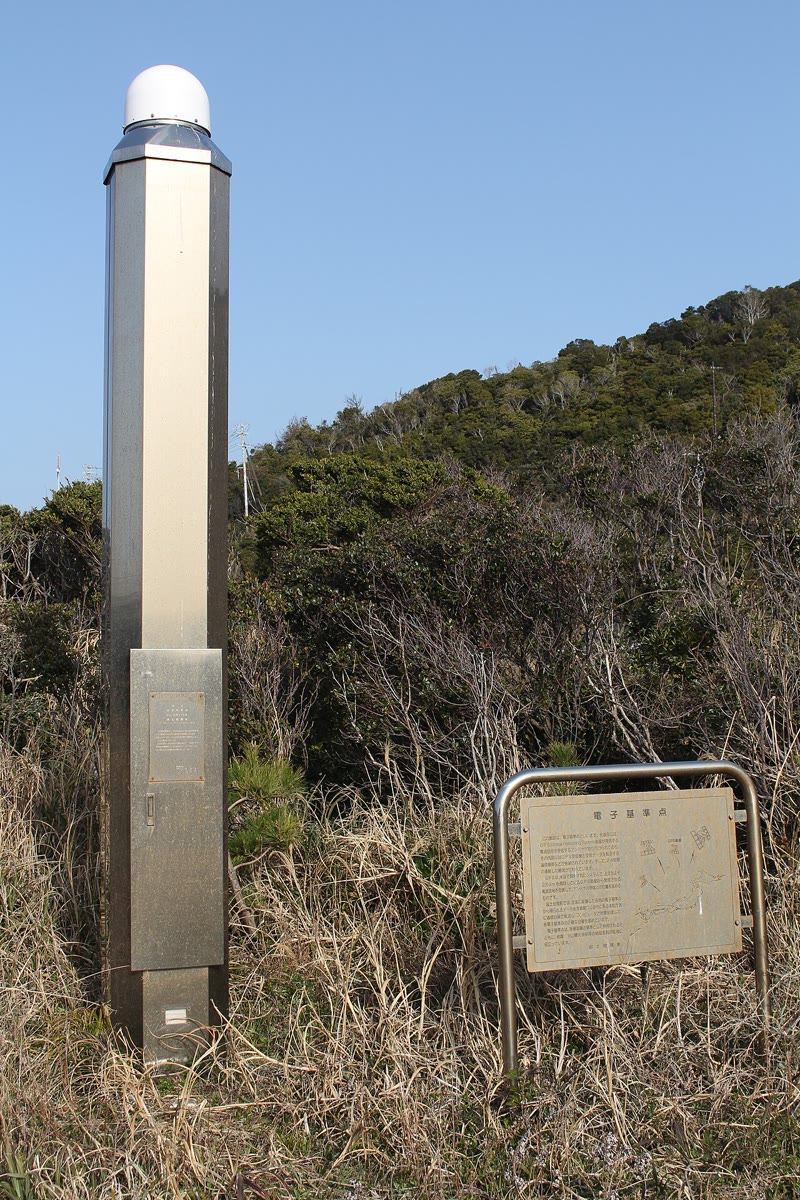
\includegraphics[width=\linewidth]{images/book3/b1-gnss-station.jpg}

{\scriptsize Een permanent station in Japan, met de antenne onder de koepel
(Alpsdake, CC BY-SA 4.0).}
\end{minipage}
\end{inthefield}

De snelheden van stations in het binnenste van twee platen geven een eigen \omterm{def:b1:plate-kinematics:euler-pole}{Eulervector}, onafhankelijk van het geologische verslag. Voor Eurazië ten opzichte van Noord-Amerika voorspelt zo'n vector \qty{17.0}{mm.yr^{-1}} op IJsland, ongeveer \qty{8}{\percent} minder dan de \qty{18.6}{mm.yr^{-1}} gemiddeld over \qty{3.16}{Myr} (figuur hierboven). De verbinding tussen Reykjavik en Stavanger, beide op stabiele delen van hun platen, wordt met \qty{17.5}{mm.yr^{-1}} langer; de satellietvector voorspelt \qty{17.1}{mm.yr^{-1}}, de geologische \qty{18.6}{mm.yr^{-1}}. Over de Noord-Atlantische Oceaan stemmen een snelheid die over enkele decennia is gemeten en een snelheid die over drie miljoen jaar is gemiddeld dus binnen een tiende van elkaar overeen: daar bewegen de platen vandaag bijna zoals zij al miljoenen jaren bewegen.
% ledger: morvel:gps-eu-na, morvel:eu-na, ngl:reyk, ngl:stas (chord rates computed in calc/ch12.py)

Binnen de grenszone is het beeld minder eenvoudig, want de stations bewegen met meer dan de platen. Meer dan een tiende van IJsland ligt onder ijskappen, en de meeste daarvan verliezen sinds ongeveer 1890 massa: de \omterm{def:b1:layered-earth:layers}{korst} eronder rijst naarmate de belasting afneemt, en beweegt horizontaal weg van het uitdunnende ijs. Het station bij Höfn, aan de zuidoostkust nabij de grootste ijskap, rijst met \qty{12.9}{mm.yr^{-1}}.
% ledger: spaans:iceland-gia, ngl:hofn

\section{Oefeningen}

Neem overal $R = \qty{6371}{km}$.

\begin{exercise}[$\star$]\label{exo:b1:plate-kinematics:1}
De \omterm{def:b1:plate-kinematics:euler-pole}{Eulervector} van Eurazië ten opzichte van Noord-Amerika heeft de snelheid \qty{0.210}{\degree\per\Myr}. (a) Reken haar om in \unit{rad.yr^{-1}} en in \unit{rad.s^{-1}}. (b) Hoe lang zou een volledige omwenteling duren? (c) Bereken $\omega R$ in \unit{mm.yr^{-1}}.
% ledger: morvel:eu-na
\end{exercise}

\begin{exercise}[$\star$]\label{exo:b1:plate-kinematics:2}
Bereken met dezelfde \omterm{def:b1:plate-kinematics:euler-pole}{Eulervector} de relatieve snelheid van de twee platen op \ang{30}, \ang{60} en \ang{90} van de \omterm{def:b1:plate-kinematics:euler-pole}{Eulerpool}. Waar langs de plaatgrens zou de spreiding het snelst zijn?
\end{exercise}

\begin{exercise}[$\star$]\label{exo:b1:plate-kinematics:3}
De normale subchron van Jaramillo duurde van \qty{1.072}{Ma} tot \qty{0.988}{Ma}. (a) Hoe breed is de streep die hij op elke flank van een rug met een \omterm{def:b1:plate-kinematics:spreading-rate}{halve spreidingssnelheid} van \qty{50}{mm.yr^{-1}} maakt? Van \qty{10}{mm.yr^{-1}}? (b) Hoe breed is de totale streep van het huidige normale chron, dat begon op \qty{0.781}{Ma}, op een rug met een halve snelheid van \qty{10}{mm.yr^{-1}}?
% ledger: iodp:gpts2004
\end{exercise}

\begin{exercise}[$\star$]\label{exo:b1:plate-kinematics:4}
Op een profiel over een rug ligt de jonge rand van de anomalie van chron C2An, \qty{2.581}{Ma} oud, \qty{66}{km} ten westen van de as en \qty{64}{km} ten oosten ervan. Bereken de twee halve spreidingssnelheden en de \omterm{def:b1:plate-kinematics:spreading-rate}{volle spreidingssnelheid}. Is de spreiding symmetrisch?
% ledger: iodp:gpts2004
\end{exercise}

\begin{exercise}[$\star\star$]\label{exo:b1:plate-kinematics:5}
Een punt van de Gakkelrug, in de Noordelijke IJszee, ligt op \ang{85}\,N, \ang{0}\,E. Bereken de hoekafstand ervan tot de \omterm{def:b1:plate-kinematics:euler-pole}{Eulerpool} van Eurazië en Noord-Amerika (\ang{61.8}\,N, \ang{139.6}\,E, \qty{0.210}{\degree\per\Myr}) en de spreidingssnelheid daar. Vergelijk met de gemeten snelheden van \qtyrange{11}{12}{mm.yr^{-1}}.
% ledger: morvel:eu-na
\end{exercise}

\begin{exercise}[$\star\star$]\label{exo:b1:plate-kinematics:6}
Op het \omterm{def:b1:plate-kinematics:triple-junction}{drievoudige knooppunt} van de Azoren, \ang{39.44}\,N, \ang{29.83}\,W, bereken (a) de hoekafstand tot de \omterm{def:b1:plate-kinematics:euler-pole}{Eulerpool} van Eurazië en Noord-Amerika, (b) de spreidingssnelheid, en (c) het \omterm{def:b1:spherical-astronomy:horizontal}{azimut} van de relatieve beweging. (d) Welke richting voorspelt men voor de transformbreuken van de rug net ten noorden van het knooppunt?
% ledger: morvel:eu-na, morvel:azores
\end{exercise}

\begin{exercise}[$\star\star$]\label{exo:b1:plate-kinematics:7}
(a) Schrijf de \omterm{def:b1:plate-kinematics:euler-pole}{Eulervectoren} $\vec\omega_{\mathrm{EU\,NA}}$ (\ang{61.8}\,N, \ang{139.6}\,E, \qty{0.210}{\degree\per\Myr}) en $\vec\omega_{\mathrm{NB\,NA}}$ (\ang{79.2}\,N, \ang{40.2}\,E, \qty{0.233}{\degree\per\Myr}) uit in cartesische componenten, in \unit{\degree\per\Myr}. (b) Leid $\vec\omega_{\mathrm{NB\,EU}}$ af, met zijn pool en zijn snelheid. (c) Waarom is dit de beste manier om de beweging van Nubië ten opzichte van Eurazië te kennen?
% ledger: morvel:eu-na, morvel:nb-na
\end{exercise}

\begin{exercise}[$\star\star$]\label{exo:b1:plate-kinematics:8}
Laat $\vec e_x$ naar \ang{0}\,N, \ang{0}\,E wijzen, $\vec e_y$ naar \ang{0}\,N, \ang{90}\,E en $\vec e_z$ naar de noordpool. Bereken met de formule van Rodrigues het beeld van $\vec e_x$ (a) door de rotatie over \ang{90} om $\vec e_z$ gevolgd door de rotatie over \ang{90} om $\vec e_x$; (b) door dezelfde twee rotaties in de omgekeerde volgorde. (c) Wat betekent dit voor de reconstructie van de vroegere posities van een plaat?
\end{exercise}

\begin{exercise}[$\star\star$]\label{exo:b1:plate-kinematics:9}
Drie platen A, B en C komen samen op een knooppunt van drie riggen. Ten opzichte van A beweegt plaat B met \qty{30}{mm.yr^{-1}} naar het oosten en plaat C met \qty{40}{mm.yr^{-1}} naar het zuiden. (a) Teken de snelheidsdriehoek. (b) Bereken de snelheid en het \omterm{def:b1:spherical-astronomy:horizontal}{azimut} van C ten opzichte van B. (c) Wat is de richting van de rug tussen B en C als die loodrecht op haar as spreidt?
\end{exercise}

\begin{exercise}[$\star\star\star$]\label{exo:b1:plate-kinematics:10}
(a) Toon aan dat het spoor van de matrix $R$ van een rotatie over $\alpha$ om elke as $1 + 2\cos\alpha$ is. (b) De matrix
\[
  R = \begin{pmatrix} 0 & 0 & 1\\ 1 & 0 & 0\\ 0 & 1 & 0\end{pmatrix}
\]
is orthogonaal met determinant $1$. Bepaal haar as, als breedte- en \omterm{def:b1:spherical-astronomy:geographic}{lengtegraad}, en haar hoek. (c) Controleer het antwoord door $R$ toe te passen op $\vec e_x$, $\vec e_y$ en $\vec e_z$.
\end{exercise}

\begin{exercise}[$\star\star\star$]\label{exo:b1:plate-kinematics:11}
Vóór de satellietpositionering werden Eulerpolen gevonden uit de richtingen van transformbreuken. (a) Toon aan dat de \omterm{def:b1:plate-kinematics:euler-pole}{Eulerpool} op de grote cirkel ligt door een punt van een transformbreuk die daar loodrecht op de breuk staat, en dat de pool dus langs $\vec t_1\times\vec t_2$ ligt, waarbij $\vec t_1$ en $\vec t_2$ eenheidsvectoren zijn langs twee transformbreuken van dezelfde grens. (b) Transformbreuken lopen onder \ang{95} nabij het \omterm{def:b1:plate-kinematics:triple-junction}{drievoudige knooppunt} van de Azoren (\ang{39.44}\,N, \ang{29.83}\,W) en onder \ang{103} op IJsland (\ang{64.5}\,N, \ang{18}\,W). De horizontale eenheidsvector op \omterm{def:b1:spherical-astronomy:geographic}{breedtegraad} $\varphi$ en \omterm{def:b1:spherical-astronomy:geographic}{lengtegraad} $\lambda$ die naar het \omterm{def:b1:spherical-astronomy:horizontal}{azimut} $\beta$ wijst is $\sin\beta\,\vec e +
\cos\beta\,\vec n$, met $\vec e = (-\sin\lambda, \cos\lambda, 0)$ en $\vec n =
(-\sin\varphi\cos\lambda, -\sin\varphi\sin\lambda, \cos\varphi)$. Bepaal de pool. (c) Hoe goed bepalen twee transforms de pool?
% ledger: morvel:eu-na
\end{exercise}

\begin{exercise}[$\star\star\star$]\label{exo:b1:plate-kinematics:12}
De oostwaartse positie van een station, elke drie maanden gedurende drie jaar, is (in millimeter, vanaf $t = 0$):
\begin{center}\small
\begin{tabular}{l*{13}{c}}
\hline
$t$ (jr) & 0 & 0.25 & 0.5 & 0.75 & 1 & 1.25 & 1.5 & 1.75 & 2 & 2.25 & 2.5 & 2.75 & 3\\
$x$ (mm) & 4 & 5 & 6 & 15 & 24 & 25 & 26 & 65 & 74 & 75 & 76 & 85 & 94\\
\hline
\end{tabular}
\end{center}
Het bestaat uit een stationaire beweging, een seizoensschommeling en een sprong veroorzaakt door een aardbeving. (a) Bereken de snelheid uit de eerste en de laatste positie. (b) Bereken de negen verschillen tussen posities precies een jaar uit elkaar, en hun mediaan. (c) Verklaar waarom de mediaan van de verschillen over één jaar een robuuste schatting van de stationaire snelheid is, en wanneer zij zou falen.
\end{exercise}

\section{Probleem: IJsland splijt}

\begin{problem}[{Weekendprobleem --- de opening van de Noord-Atlantische Oceaan over IJsland,
drie keer gemeten}]
\label{pb:b1:plate-kinematics:1}
% values: calc/ch12.py (Part II profile invented for the problem; real Euler
% vectors, chron ages and station velocities)
% ledger: morvel:eu-na, morvel:nb-na, iodp:gpts2004, ngl:reyk, ngl:stas, ngl:hofn
IJsland ligt op de Mid-Atlantische Rug, tussen de Noord-Amerikaanse plaat in het westen en de Euraziatische plaat in het oosten. Neem $R = \qty{6371}{km}$ en, voor Eurazië ten opzichte van Noord-Amerika, de \omterm{def:b1:plate-kinematics:euler-pole}{Eulervector} met zijn pool op
\ang{61.8}\,N, \ang{139.6}\,E en de snelheid \qty{0.210}{\degree\per\Myr}.

\medskip
\noindent\textbf{Deel I --- De plaatvector.}
\begin{enumerate}
  \item Reken de snelheid om in \unit{rad.yr^{-1}} en bereken $\omega R$ in \unit{mm.yr^{-1}}.
  \item Bereken de hoekafstand $\Delta$ van de pool tot het midden van IJsland, \ang{64.5}\,N, \ang{18}\,W.
  \item Leid de \omterm{def:b1:plate-kinematics:spreading-rate}{volle spreidingssnelheid} over IJsland af die door de plaatvector wordt voorspeld.
  \item Bereken het \omterm{def:b1:spherical-astronomy:horizontal}{azimut} van de pool, gezien vanaf IJsland, en het \omterm{def:b1:spherical-astronomy:horizontal}{azimut} van de beweging van Eurazië ten opzichte van Noord-Amerika.
  \item Splits deze snelheid in haar oostelijke en noordelijke componenten.
  \item Op de Gakkelrug, op \ang{86}\,N, \ang{60}\,E: welke snelheid geeft dezelfde vector? Waarom is de grens daar zoveel trager?
\end{enumerate}

\noindent\textbf{Deel II --- De magnetische strepen.}
Een magnetisch scheepsprofiel over de Reykjanes-rug, ten zuidwesten van IJsland nabij \ang{63}\,N, \ang{23}\,W, gevaren in de richting van de spreiding, geeft de volgende afstanden van de as tot drie chrongrenzen (een profiel dat voor dit probleem is opgesteld):
\begin{center}\small
\begin{tabular}{lccc}
\hline
grens & leeftijd (Ma) & ten westen van de as (km) & ten oosten van de as (km)\\
\hline
basis van C1n & 0.781 & 9.7 & 10.1\\
jonge rand van C2An & 2.581 & 26.8 & 27.3\\
jonge rand van C5n & 9.779 & 94 & 97\\
\hline
\end{tabular}
\end{center}
\begin{enumerate}[resume]
  \item Bereken vanaf de jonge rand van C5n de twee halve spreidingssnelheden.
  \item Leid de \omterm{def:b1:plate-kinematics:spreading-rate}{volle spreidingssnelheid} sinds \qty{9.8}{Ma} af.
  \item Bereken de volle snelheid ook uit de twee jongere grenzen. Komen de drie overeen? Beschrijf hoe zij veranderen met de leeftijd van de grens.
  \item Is de spreiding symmetrisch? Verandert de asymmetrie de volle snelheid?
  \item Op de Reykjanes-rug zijn de grenzen tussen de strepen naar buiten van de as verschoven met in totaal \qty{5.0}{km}, beide flanken samen. Corrigeer de drie volle snelheden. Waarom was de correctie het belangrijkst voor de jongste grens?
  \item Hoe breed is de streep van de Jaramillo-subchron (\qtyrange{1.072}{0.988}{Ma}) op elke flank, bij de gecorrigeerde halve snelheid? Vergelijk met de verschuiving van vraag 11. De Jaramillo-anomalie is toch duidelijk herkend op de profielen van de Reykjanes-rug, maar ontbreekt op de Gakkelrug: wat suggereert dat?
  \item De plaatvector voorspelt \qty{19.0}{mm.yr^{-1}} bij het profiel. Vergelijk met de gecorrigeerde snelheden.
\end{enumerate}

\noindent\textbf{Deel III --- De satellieten.}
De permanente stations REYK (Reykjavik, \ang{64.139}\,N, \ang{21.955}\,W) en STAS (Stavanger, \ang{59.018}\,N, \ang{5.599}\,E) liggen op de Noord-Amerikaanse en de Euraziatische plaat. Hun gemeten snelheden maken de verbinding ertussen met \qty{17.5}{mm.yr^{-1}} langer.
\begin{enumerate}[resume]
  \item Bereken de hoekafstand tussen de twee stations, en de lengte van de verbinding.
  \item Hoe lang duurt het voordat de verbinding met één meter is langer geworden?
  \item De plaatvector geeft STAS een snelheid van \qty{18.9}{mm.yr^{-1}} naar \ang{114.8} ten opzichte van Noord-Amerika. De grote cirkel vanaf REYK komt bij STAS aan met een richting naar \ang{123.1}. Bereken de component van de snelheid langs deze richting, en daarna de voorspelde verlenging van de verbinding, die met de horizontaal bij STAS de hoek $\Delta/2$ maakt.
  \item Vergelijk de gemeten en de voorspelde verlenging. Wat zou het verschil kunnen verklaren?
  \item Ten opzichte van Noord-Amerika beweegt REYK met \qty{1.07}{mm.yr^{-1}} naar het westen en \qty{0.97}{mm.yr^{-1}} naar het zuiden, en het station HOFN (Höfn, zuidoost-IJsland) met \qty{21.12}{mm.yr^{-1}} naar het oosten en \qty{6.97}{mm.yr^{-1}} naar het zuiden. Bereken de snelheid en het \omterm{def:b1:spherical-astronomy:horizontal}{azimut} van HOFN ten opzichte van REYK.
  \item Vergelijk met deel I. HOFN rijst ook met \qty{12.9}{mm.yr^{-1}}. Waarom zijn stations binnen IJsland een slechte maat voor de beweging van de platen?
\end{enumerate}

\noindent\textbf{Deel IV --- Tien miljoen jaar, en het knooppunt in het zuiden.}
\begin{enumerate}[resume]
  \item Over \qty{10}{Myr}, over welke hoek draait Eurazië ten opzichte van Noord-Amerika om de pool?
  \item Hoe ver reist een punt van Eurazië in het midden van IJsland in die tijd langs zijn \omterm{def:b1:spherical-astronomy:spherical-triangle}{kleine cirkel}? Vergelijk met de gecorrigeerde breedte van de \omterm{def:b1:layered-earth:layers}{korst} die is gevormd sinds de jonge rand van C5n in deel II.
  \item Op het \omterm{def:b1:plate-kinematics:triple-junction}{drievoudige knooppunt} van de Azoren geven de plaatvectoren aan Eurazië \qty{22.9}{mm.yr^{-1}} naar \ang{95.1} en aan Nubië \qty{19.2}{mm.yr^{-1}} naar \ang{103.8}, beide ten opzichte van Noord-Amerika. Bereken de snelheid van Eurazië ten opzichte van Nubië.
  \item Is dit knooppunt stabiel? Wat voor soort grens impliceert de snelheid van vraag 22 tussen Eurazië en Nubië?
  \item Verzamel de openingssnelheden van de delen I, II en III. Welke stemmen overeen, en welke methode meet de beweging van de platen over de kortste tijd?
  \item Op het dichtstbijzijnde millimeter per jaar: welke \omterm{def:b1:plate-kinematics:spreading-rate}{volle spreidingssnelheid} over IJsland geven de plaatvector en de gecorrigeerde magnetische strepen beide?
\end{enumerate}
\end{problem}
